\documentclass[a4paper,12pt]{article}
\usepackage{amsmath, amssymb, xcolor, tcolorbox}
\usepackage{geometry}
\usepackage{enumitem}
\usepackage{fancyhdr}
\usepackage{graphicx}
\usepackage{multicol}
\geometry{top=1in, bottom=1in, left=1in, right=1in}    % Header and Footer settings
\pagestyle{plain}
\begin{document}
\thispagestyle{fancy}
\fancyhf{} % Clear default header and footer
\fancyhead[L]{
	
\includegraphics[width=8cm, height=1.7cm]{IIITB-COMET-Logo.png}
}
\fancyhead[R]{
	Name: N.SRINIVAS \\
	Batch: COMETFWC036 \\
	Date: 12 August 2025
}
\renewcommand{\headrulewidth}{0pt} % Remove header line
\fancyfoot[C]{\thepage} % Page number centered in footer
\vspace*{0.1em}
\begin{center}
\section*{\textbf{\huge GATE, EE 2010}}
\end{center}
\begin{itemize}[label={}, leftmargin=0pt]
	\item $11$. Match the logic gates in \textbf{Column A} with their equivalents in \textbf{Column B.}
\begin{center}
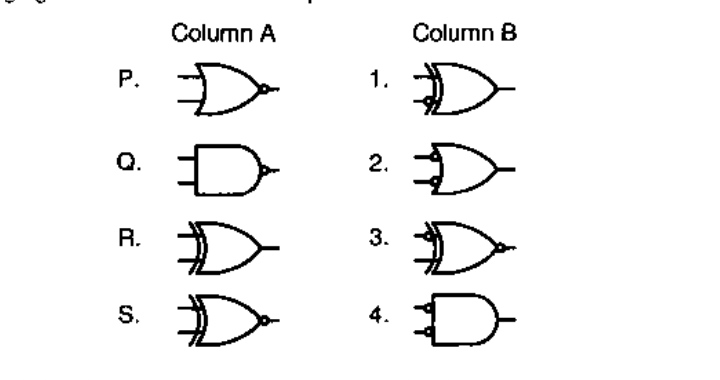
\includegraphics[width=15cm, height=10cm]{circuit.jpg}
\end{center}
	\begin{multicols}{2}
		\begin{enumerate}[label=\Alph*]
			\item P-2, Q-4, R-1, S-3
			\item P-4, Q-2, R-1, S-3 
			\item P-2, Q-4, R-3, S-1  
			\item P-4, Q-2, R-3, S-1
		\end{enumerate}
	\end{multicols}
\section*{\textbf{\large SOLUTION: }}
	\item Let $X$ and $Y$ be the inputs, $Z$ be the output for each logic gate in Column A and Column B.
	\item \textbf{The output expressions of each gate in Column A as follows:}
	\item For P - $>$ $Z$ = $\overline{X+Y}$
	\item For Q - $>$ $Z$ = $\overline{X.Y}$
	\item For R - $>$ $Z$ = $X \oplus Y$
	\item For S - $>$ $Z$ = $X \odot Y$
	\item \textbf{The output expressions of each gate in Column B as follows:}
	\item For 1 - $>$ $Z$ = $X \oplus \bar{Y}$ = $X.\bar{\bar{Y}}+\bar{X}.\bar{Y}$ = $X.Y+\bar{X}.\bar{Y}$ = $X \odot Y$
	\item For 2 - $>$ $Z$ = $\bar{X} + \bar{Y}$ = $\overline{X.Y}$
	\item For 3 - $>$ $Z$ = $\bar{X} \odot Y$ = $\bar{X}.Y+\bar{\bar{X}}.\bar{Y}$ = $\bar{X}.Y+X.\bar{Y}$ = $X \oplus Y$
	\item For 4 - $>$ $Z$ = $\bar{X} . \bar{Y}$ = $\overline{X+Y}$
	\item Hence From above Expression the correct Match is \textbf{P-4, Q-2, R-3, S-1}. So the final correct option is \textbf{$D$}.
	\item \textbf{\large ANS: Option D}
\end{itemize}
\end{document}
